\documentclass[conference]{IEEEtran}
\usepackage{graphicx}

\title{Measurement of Fetal Head Circumference using Ultrasound}
\author{Nguyen Son}
\begin{document}

\maketitle

\begin{abstract}
    This report is not using GPT or anything fancy, it's just a simple report about Measurement of Fetal Head Circumference using Ultrasound. I will introduce you to the project, then I will talk about the background, the method, the results, the discussion, and the conclusion. I hope you enjoy it.
\end{abstract}

\section{Introduction}
This is the Introduction which I will write out the definition for things and introduce you to the project.

\subsection{Ultrasound}
Ultrasound is a non-invasive imaging technique that uses high-frequency sound waves to produce images of structures within the body. It is commonly used in pregnancy to evaluate the development and health of the fetus. (https://www.radiologyinfo.org/en/info/obstetricus)

\subsection{Fetal Head Circumference (HC)}
Fetal head circumference is a key measurement taken during ultrasound examinations to assess the size and growth of the fetus. It is crucial for determining gestational age, diagnosing potential anomalies, and monitoring the health and development of the fetus. (https://radiopaedia.org/articles/head-circumference)

\subsection{Importance of HC Measurement}
The measurement of fetal head circumference is significant as it provides essential information about fetal growth patterns and can help in the early detection of growth restrictions or macrocephaly. It is a fundamental component of prenatal care.

\subsection{Ultrasound in Obstetrics}
Ultrasound in obstetrics is dedicated to the use of ultrasound imaging in pregnancy, providing detailed views of the fetus and uterus, which help in monitoring the health and development of the fetus. It plays a critical role in routine prenatal care.

\subsection{Technological Advances in Ultrasound}
With advancements in technology, ultrasound machines have become more sophisticated, offering clearer images and enabling more accurate measurements of fetal parameters, including head circumference. This progress has enhanced the diagnostic capabilities of prenatal ultrasound.

\subsection{Challenges in Measuring Fetal HC}
Accurately measuring fetal head circumference can be challenging due to fetal position, movements, and the skill level of the sonographer. Addressing these challenges is crucial for ensuring accurate assessments of fetal well-being.

\subsection{Objectives}
The objective of this project is to explore the techniques and importance of measuring fetal head circumference using ultrasound, addressing the challenges faced during this process and discussing the implications of accurate measurements for prenatal care and fetal health assessment.

\section{Method}
I use U-Net which is a simple encode-decode Convolutional Neural Network (CNN) model. It's a good model.

\section{Results}
First I visualize the training session.
\begin{figure}[h]
    \centering
    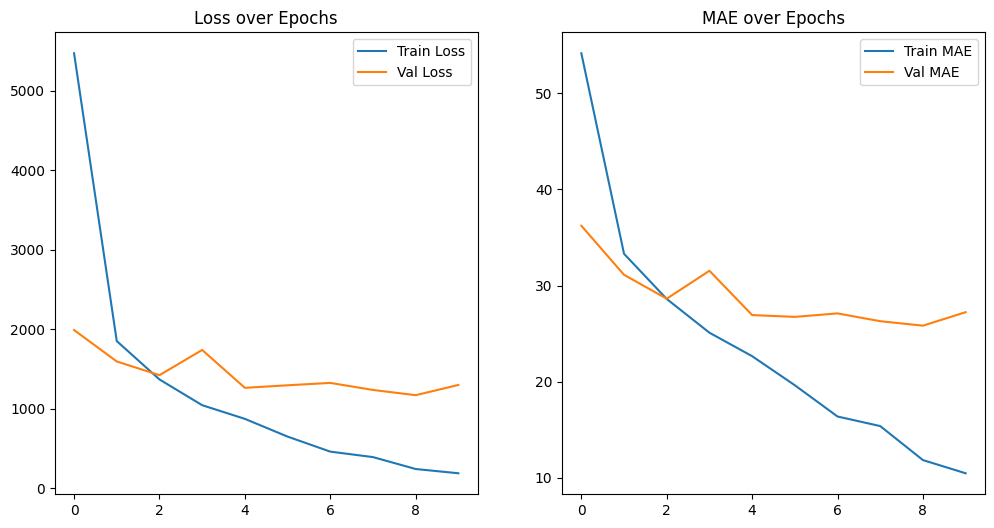
\includegraphics[width=\linewidth]{eva1.png}
    \caption{Epochs Visualization}
    \label{fig:Epochs Visualization}
\end{figure}
it looks good i guess?

Then I make this mess
\begin{figure}[h]
    \centering
    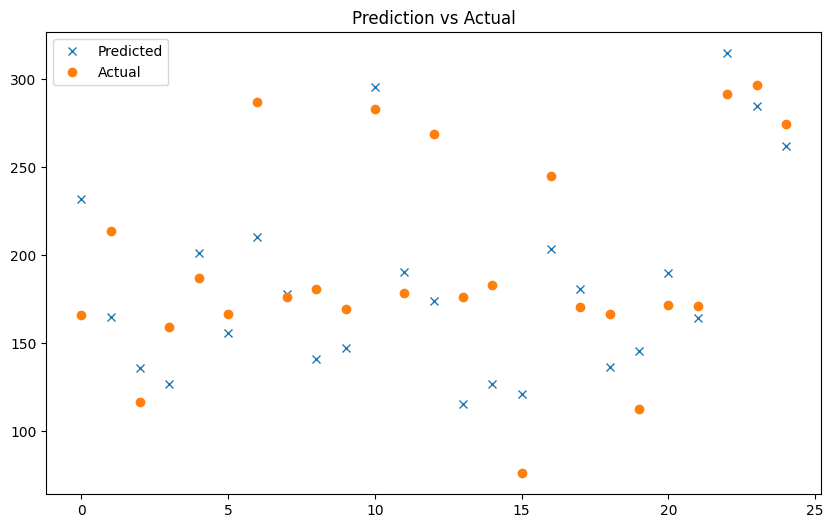
\includegraphics[width=\linewidth]{eva2.png}
    \caption{Prediction vs Actual}
    \label{fig:Prediction vs Actual}
\end{figure}
which I really don't know how to comment on.

Finally, I make this Prediction Error Distribution
\begin{figure}[h]
    \centering
    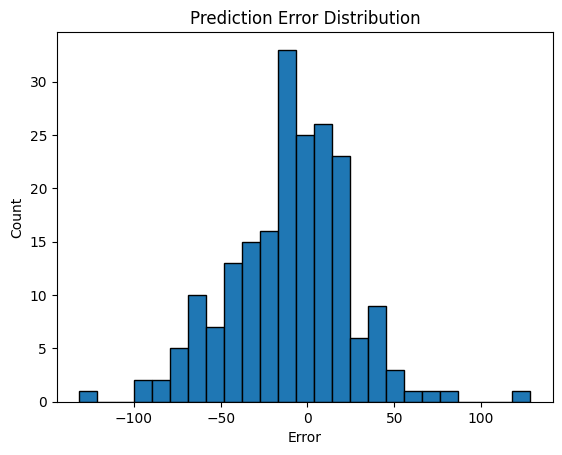
\includegraphics[width=\linewidth]{eva3.png}
    \caption{Prediction Error Distribution}
    \label{fig:Prediction Error Distribution}
\end{figure}
which it also said the Mean Absolute Error is 27.22 mm.

\section{Discussion}
The model ran good. I think it's good. I don't know what else to say.

\section{Conclusion}
Google Colab without Pro sucks.

\end{document}
